\documentclass[a4paper,11pt]{article}
\usepackage{amsmath,amssymb}
\usepackage{graphicx}

\title{Modelling and Simulation I\\Exercises 4.2 and 4.3}
\author{}
\date{}

\begin{document}
\maketitle

\section*{4.2 Statistical counters for correlations}

For a series of \(n\) samples with mean \(\bar{x}\), the counter estimates
\[
\widehat{\gamma}(k)=
\frac{1}{n-k}\sum_{i=1}^{n-k}(x_i-\bar{x})(x_{i+k}-\bar{x}),
\qquad
\widehat{r}(k)=\frac{\widehat{\gamma}(k)}{\widehat{\gamma}(0)}.
\]
Lag \(k\) compares observations \(k\) positions apart. The
autocovariance averages the products of their deviations from the
mean. A positive value means that deviations to the same side of the
mean tend to dominate, while a negative value means that opposite
deviations tend to dominate. Lag-zero covariance is the average
squared deviation from the mean, in squared units of the samples.
Dividing by this value makes autocorrelation unitless. A lag without
sample pairs is undefined, and autocorrelation is undefined when the
lag-zero covariance is zero.

Each validation series contains 12,000 samples. The first six values
are shown below. The Gaussian-based values are rounded to three
decimal places and were generated with seed 42.

\begin{center}
\small
\begin{tabular}{ll}
\hline
Series & First six samples \\
\hline
Constant \(2\) & \(2,\,2,\,2,\,2,\,2,\,2\) \\
Repeating \(2,2,-2\) & \(2,\,2,\,-2,\,2,\,2,\,-2\) \\
Alternating \(1,-1\) & \(1,\,-1,\,1,\,-1,\,1,\,-1\) \\
Increasing ramp & \(0,\,1,\,2,\,3,\,4,\,5\) \\
Gaussian white noise & \(0.919,\,-0.950,\,-1.107,\,0.281,\,0.685,\,-0.817\) \\
Two-sample moving average & \(1.031,\,-0.015,\,-1.028,\,-0.413,\,0.483,\,-0.066\) \\
\hline
\end{tabular}
\end{center}

The numbered columns in the next table show the autocorrelation
at the corresponding lag.

\begin{center}
\small
\setlength{\tabcolsep}{4pt}
\begin{tabular}{lrrrrrrr}
\hline
Series & \(\widehat{\gamma}(0)\) & 1 & 2 & 3 & 4 & 5 & 6 \\
\hline
Constant \(2\) & 0 & -- & -- & -- & -- & -- & -- \\
Repeating \(2,2,-2\) & 3.556 & -.500 & -.500 & 1 & -.500 & -.500 & 1 \\
Alternating \(1,-1\) & 1 & -1 & 1 & -1 & 1 & -1 & 1 \\
Increasing ramp & \(1.20 \cdot 10^7\) & 1.000 & 1.000 & .999 & .999 & .999 & .999 \\
Gaussian white noise & .992 & .008 & .011 & -.001 & -.006 & -.018 & .011 \\
Two-sample moving average & .500 & .509 & .014 & .001 & -.015 & -.015 & .005 \\
\hline
\end{tabular}
\end{center}

The constant series has zero covariance because every sample equals
the mean. The period-three series has correlation near \(-0.5\) at
lags 1 and 2, where the negative cross-products outweigh the positive
ones. It realigns at lags 3 and 6, giving a correlation of 1.
For the alternating series, every pair at an odd lag has opposite
signs, giving \(-1\), and every pair at an even lag has matching signs,
giving \(1\). In the ramp, samples a few positions apart have nearly
the same deviation from the mean. The trend produces correlations
close to 1 over these lags.

The white-noise correlations fluctuate around zero. Adjacent samples
in the moving average share one noise value, giving a theoretical
lag-1 correlation of 0.5 and an observed value of 0.509. At higher
lags the pairs share no noise values and the estimates are close to zero.

\section*{4.3 M/M/1 queue simulation}

\subsection*{Mean waiting times}

Interarrival and service times are exponential. Utilization is
\(\rho = \mathbb{E}[S]/\mathbb{E}[A]\), so with a mean interarrival
time of \(1\,\mathrm{s}\), the required mean service time is
\(0.80\,\mathrm{s}\) at 80\% and \(0.95\,\mathrm{s}\) at 95\%.
Both runs start with an empty queue and reuse the same random seeds.
Waiting time is measured from arrival to the start of service.

\begin{center}
\begin{tabular}{lrrr}
\hline
Utilization & First 10 & First 100,000 & Steady-state mean \\
\hline
80\% & \(4.944\,\mathrm{s}\) & \(3.237\,\mathrm{s}\) & \(3.200\,\mathrm{s}\) \\
95\% & \(6.446\,\mathrm{s}\) & \(18.686\,\mathrm{s}\) & \(18.050\,\mathrm{s}\) \\
\hline
\end{tabular}
\end{center}

Each mean is the total time spent in the queue divided by the number
of customers, including customers who waited zero seconds. The first
ten waits are sensitive to the empty initial queue and to individual
early arrivals and service times. At 80\%, the early mean of
\(4.944\,\mathrm{s}\) exceeds the 100,000-customer mean by
\(1.707\,\mathrm{s}\). At 95\%, the early mean is about
\(12.240\,\mathrm{s}\) below the longer-run mean. Both longer-run
estimates are closer to the theoretical steady-state mean
\(\mathbb{E}[W_q]=\rho\mathbb{E}[S]/(1-\rho)\).
Increasing utilization from 80\% to 95\% raised the measured
100,000-customer mean wait by a factor of about 5.8.

\subsection*{Waiting-time histograms}

\begin{center}
\begin{minipage}{\textwidth}
\centering
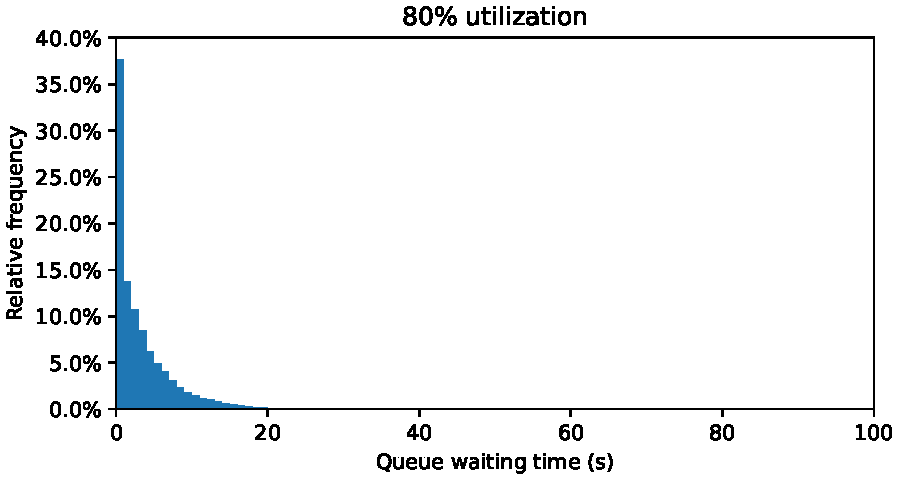
\includegraphics[width=0.8\linewidth]{plots/waiting-time-rho80.pdf}
\par
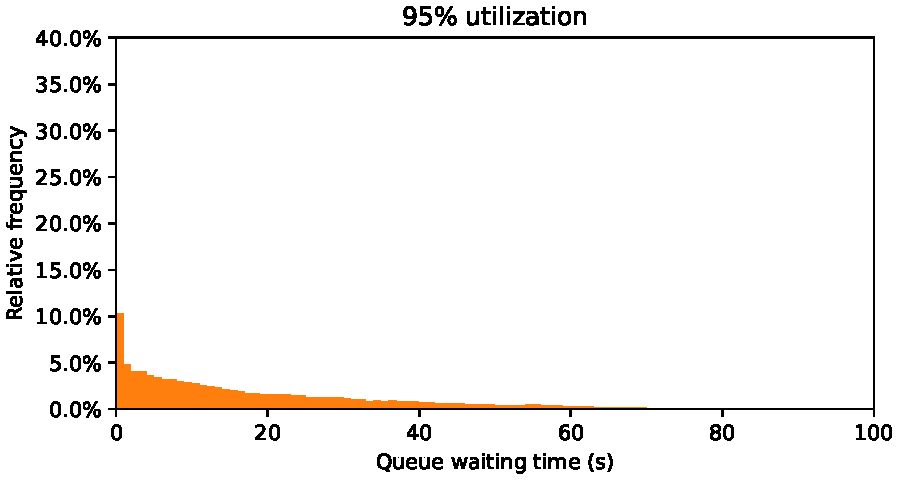
\includegraphics[width=0.8\linewidth]{plots/waiting-time-rho95.pdf}
\end{minipage}
\end{center}

Each bar is the percentage of the 100,000 customers whose wait fell
into that one-second interval. The same vertical scale is used in
both plots. At 80\%, 37.651\% waited less than one second, compared
with 10.264\% at 95\%. These first bins include the customers who
started service immediately, who account for 20.137\% and 5.374\%
of the respective runs. At 95\%, 7.612\% waited at least 50 seconds,
compared with none at 80\%. The final bin contains all waits of
99 seconds or more. With less idle capacity to clear the queue,
the 95\% run has more long waits.

\subsection*{Waiting-time autocorrelation}

\begin{center}
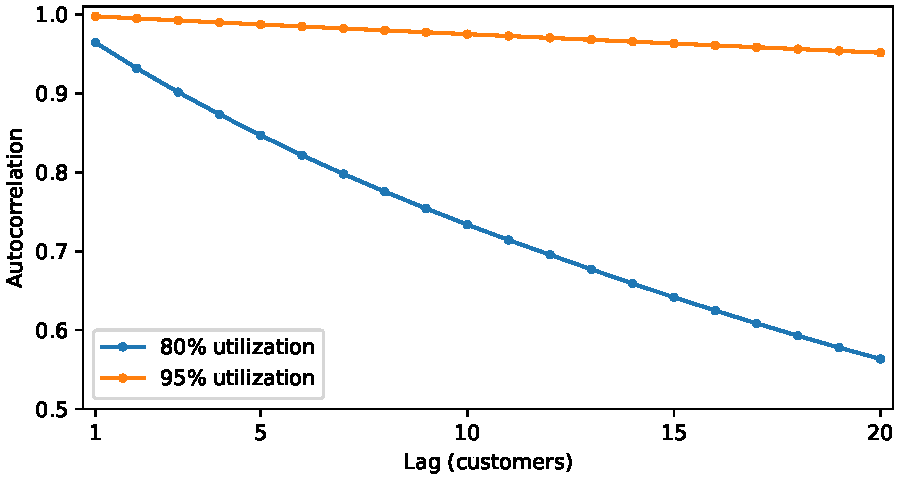
\includegraphics[width=0.85\textwidth]{plots/waiting-time-autocorrelation.pdf}
\end{center}

\begin{center}
\small
\begin{tabular}{rrr@{\qquad}rrr}
\hline
Lag & 80\% & 95\% & Lag & 80\% & 95\% \\
\hline
 1 & .9641 & .9973 & 11 & .7141 & .9723 \\
 2 & .9314 & .9947 & 12 & .6954 & .9700 \\
 3 & .9014 & .9921 & 13 & .6771 & .9676 \\
 4 & .8732 & .9895 & 14 & .6590 & .9652 \\
 5 & .8466 & .9870 & 15 & .6416 & .9629 \\
 6 & .8214 & .9844 & 16 & .6248 & .9605 \\
 7 & .7978 & .9819 & 17 & .6086 & .9582 \\
 8 & .7753 & .9795 & 18 & .5929 & .9558 \\
 9 & .7541 & .9771 & 19 & .5778 & .9535 \\
10 & .7336 & .9747 & 20 & .5636 & .9512 \\
\hline
\end{tabular}
\end{center}

Lag 1 compares each customer's wait with the next customer's wait.
Lag 20 compares it with the wait of the customer 20 positions later.
At 80\%, the correlation falls from 0.964 at lag 1 to 0.564 at lag 20.
At 95\%, it falls from 0.997 to 0.951. The value 0.951 is unitless
and indicates that even 20 positions later, above-average waits tend
to occur together, as do below-average waits. With only 5\% spare
capacity, a backlog takes longer to clear and affects more successive
customers.

The lag-zero covariance rises from \(15.806\,\mathrm{s}^2\) to
\(326.719\,\mathrm{s}^2\). Its square root gives a standard deviation
of about \(3.98\,\mathrm{s}\) at 80\% and \(18.08\,\mathrm{s}\) at 95\%.
The higher-utilization run has both a wider spread of waits and a
slower decay in dependence between successive waits.

\end{document}
